\documentclass[12pt,a4paper]{article}
		\usepackage{amsmath}
		\usepackage{amsfonts}
		\usepackage{amssymb}
		\usepackage{pgf,tikz}
		\usepackage{mathrsfs}
		\usepackage{adjustbox}
		\usepackage{tabularx}
		\usepackage{multicol}
		\usepackage{etex}
		\usepackage{circuitikz}
		\usetikzlibrary {circuits.ee.IEC}
		\usepackage{pgf}
		\usepackage{bm}
		\usepackage{pstricks}
		\let\clipbox\relax
		\usetikzlibrary{arrows}
		\usepackage{lastpage}
		\usepackage{setspace}
		\usepackage{enumitem}
		\usepackage{graphicx} %table
		\usepackage{diagbox}
		\usepackage[left=1.5cm,right=1.5cm,top=1.5cm,bottom=1.5cm,includehead,includefoot]{geometry}
		\usepackage{xcolor}
		\usepackage{polyglossia}
		\usepackage{graphicx}
		\usepackage[most]{tcolorbox}
		\usepackage{titlesec}
		\usepackage{fancyhdr} % Mise en page, en-tête et pied de page
		\usepackage[a4,frame,center]{crop}
		\setdefaultlanguage[calendar=gregorian,numerals=maghrib]{arabic}
		\setotherlanguage{french}
		\newfontfamily\arabicfont[Script=Arabic,Scale=1]{Amiri}
		\newfontfamily\arabicfontsf[Script=Arabic,Scale=1]{Amiri}
		\newtcbtheorem[auto counter]{exercice}%
		{\textbf{تمرين}}{enhanced jigsaw,breakable,before skip=1mm,after skip=1mm,/tcb/bottom= 1 mm ,/tcb/top= 1 mm ,
		attach boxed title to top right={xshift=-1cm,yshift=-3mm},
		fonttitle=\bfseries,varwidth boxed title=0.7\linewidth,
		colbacktitle=white!45!white,coltitle=white!10!black,colframe=white!50!black,
		interior style={top color=white!10!white,bottom color=blue!10!white},
		boxed title style={boxrule=0.3mm,colframe=white,
		borderline={0.1mm}{0mm}{blue!50!black},
		borderline={0.1mm}{0.4mm}{blue!50!black},
		interior style={top color=white!10!white,bottom color=white!10!white,
		middle color=blue!10!white},
		drop fuzzy shadow,arc=0mm},arc=0mm, colback=white!5!white,colframe=blue!50!white}{theorem}
		%Solution ==================================================
		\newtcbtheorem[]{solution}%
		{\textbf{حل التمرين}}{enhanced jigsaw,breakable,/tcb/top=4mm,before skip=1mm,after skip=1mm,
		attach boxed title to top center={xshift=0cm,yshift=-3.7mm},
		fonttitle=\bfseries,varwidth boxed title=0.7\linewidth,
		colbacktitle=white!45!white,coltitle=white!10!black,colframe=white!50!black,
		interior style={top color=white!10!white,bottom color=blue!10!white},
		boxed title style={boxrule=0.5mm,
		frame code={ \path[tcb fill frame] ([xshift=-4mm]frame.west)
		-- (frame.north west) -- (frame.north east) -- ([xshift=4mm]frame.east)
		-- (frame.south east) -- (frame.south west) -- cycle; },
		interior code={ \path[tcb fill interior] ([xshift=-2mm]interior.west)
		-- (interior.north west) -- (interior.north east)
		-- ([xshift=2mm]interior.east) -- (interior.south east) -- (interior.south west)
		-- cycle;} }
		,arc=0mm, colback=white!5!white,colframe=blue!50!white}{theorem}
		%============================================================
		\setlength{\columnseprule}{1pt}
		\def\columnseprulecolor{\color{blue}}
		\titlespacing{\section}{0pt}{0pt}{0pt}
		\titlespacing{\section}{0pt}{0pt}{0pt}
		\pagestyle{fancy}
		\cfoot{\thepage}
		%\rfoot{}
		\definecolor{color1}{RGB}{0,0,0}
		\newcommand*\circled[1]{\tikz[baseline=(char.base)]{%
        \node[shape=circle,left color=color1!60!black,right color=color1!60!black,
		middle color=color1!80!black,draw,inner sep=1pt] (char) {#1};}}
		%==============================
		\newcommand*\rectled[1]{\tikz[baseline=(char.base)]{%
        \node[shape=rectangle,left color=color1!60!black,right color=color1!60!black,
		middle color=color1!80!black,draw,inner sep=1pt] (char) {#1};}}
		\lfoot{السنة الدراسية : 
  }
\lhead{مادة : الفيزياء والكيمياء\\الأستاذ :  }
\rhead{الثانوية التأهيلية  : \\المستوى الدراسي  :  }
\rfoot{أمثلة لثأثيرات ميكانيكية  }
\lfoot{}
 \chead{\centering سلسلة تمارين\\ 
أمثلة لثأثيرات ميكانيكية  }
\begin{document}
  
  %Exercice 1
\begin{exercice}{}/
					\textbf{\begin{minipage}[c]{0.74\linewidth}
					يطبق الخيط على الجسم 
					$\bm{(S)}$
					ذي الكتلة 
					$\bm{m=200\ g}$
					قوة 
					$\bm{{\overrightarrow{T}}}$
					شدتها
					$\bm{T = 2\ N}$.
					\begin{enumerate}[label=\protect\circled{\color{white}\textbf{\arabic*}}]
					\item أجرد القوى المطبقة على الجسم 
					$\bm{(S)}$
					وصنفها.
					\item أعط مميزات كل قوة.
					\item باستعمال السلم
					$\bm{{1cm\ \longrightarrow\ 1N}}$
					مثل هذه القوى.
					\end{enumerate}
					نعطي
					$\bm{g=10\ N.kg^{-1}}$.}
					\end{minipage}
					\begin{minipage}[c]{0.24\linewidth}
\definecolor{cffffff}{RGB}{255,255,255}
\definecolor{cffaf00}{RGB}{255,175,0}
\begin{flushleft}
\begin{adjustbox}{width=0.8\linewidth}
\fbox{
\begin{tikzpicture}[y=0.80pt, x=0.80pt, yscale=-1.000000, xscale=1.000000, inner sep=0pt, outer sep=0pt]
\begin{scope}[shift={(-374.5,-77.5)}]
  \path[shift={(375.5,78.5)},draw=black,fill=cffffff] (0.0000,0.0000) --
    (205.5000,0.0000) -- (205.5000,297.0000) -- (0.0000,297.0000) --
    (0.0000,0.0000) -- cycle;
  \path[shift={(484.0,94.0)},draw=black,fill=black] (0.0000,0.0000) --
    (71.0000,0.0000) -- (71.0000,5.0000) -- (0.0000,5.0000) -- (0.0000,0.0000) --
    cycle;
  \path[cm={{0.01,1.0,-1.0,0.01,(519.5,99.0)}},draw=black,line width=2.133pt]
    (0.0000,0.0000) -- (194.0000,0.0000);
  \path[shift={(489.0,293.0)},draw=black,fill=cffaf00,line width=2.133pt]
    (0.0000,33.0000) .. controls (0.0000,14.8000) and (14.8000,0.0000) ..
    (33.0000,0.0000) .. controls (51.2000,0.0000) and (66.0000,14.8000) ..
    (66.0000,33.0000) .. controls (66.0000,51.2000) and (51.2000,66.0000) ..
    (33.0000,66.0000) .. controls (14.8000,66.0000) and (0.0000,51.2000) ..
    (0.0000,33.0000) -- cycle;
  \begin{scope}[shift={(394.7,205.27)}]
    \path (38,13) node[] (text14) {\Large \textbf{خيط}};
  \end{scope}
  \begin{scope}[shift={(394.7,312.77)}]
    \path (38,13) node[] (text14) {\Large $(S)$};
  \end{scope}
  \begin{scope}[shift={(470.3,218.9)}]
    \path[draw=black,line width=2.133pt] (0.0000,0.0000) -- (42.5000,0.0000);
    \path[draw=black,fill=black,line cap=round,line width=0.800pt] (49.7000,0.0000)
      -- (41.2000,-4.9000) .. controls (42.1000,-3.5000) and (42.5000,-1.8000) ..
      (42.5000,0.0000) .. controls (42.5000,1.8000) and (42.1000,3.5000) ..
      (41.2000,4.9000) -- (49.7000,0.0000);
  \end{scope}
  \begin{scope}[cm={{1.0,-0.02,0.02,1.0,(470.3,326.4)}}]
    \path[draw=black,line width=2.133pt] (0.0000,0.0000) -- (11.5000,0.0000);
    \path[draw=black,fill=black,line cap=round,line width=0.800pt] (18.7000,0.0000)
      -- (10.2000,-4.9000) .. controls (11.1000,-3.5000) and (11.5000,-1.8000) ..
      (11.5000,0.0000) .. controls (11.5000,1.8000) and (11.1000,3.5000) ..
      (10.2000,4.9000) -- (18.7000,0.0000);
  \end{scope}
  \begin{scope}[shift={(394.7,115.54)}]
    \path (38,13) node[] (text14) {\Large \textbf{حامل}};
  \end{scope}
  \path[shift={(470.3,129.17)},draw=black,line width=2.133pt] (0.0000,0.0000) --
    (20.7000,0.0000);
  \begin{scope}[cm={{0.37,-0.93,0.93,0.37,(491.3,128.0)}}]
    \path[draw=black,line width=2.133pt] (0.0000,0.0000) -- (24.1000,0.0000);
    \path[draw=black,fill=black,line cap=round,line width=0.800pt] (31.3000,0.0000)
      -- (22.8000,-4.9000) .. controls (23.6000,-3.5000) and (24.1000,-1.8000) ..
      (24.1000,0.0000) .. controls (24.1000,1.8000) and (23.6000,3.5000) ..
      (22.8000,4.9000) -- (31.3000,0.0000);
  \end{scope}
\end{scope}
\end{tikzpicture}}
\end{adjustbox}
\end{flushleft}
					\end{minipage}
					\end{exercice}%=== source ===%
  %Exercice 2
\begin{exercice}{}/
\definecolor{cffffff}{RGB}{255,255,255}
\definecolor{cffaf00}{RGB}{255,175,0}
\definecolor{c3498db}{RGB}{52,152,219}
					\textbf{يتحرك جسم صلب 
					$\bm{(S)}$
					فوق سطح مستوي، الأشكال أسفله تمثل أوضاعا مختلفة لهذا الجسم، في أي حالة يتم التماس باحتكاك؟وفي أي حالة يتم التماس بدون احتكاك؟ علل جوابك؟\\
					\begin{minipage}[c]{0.24\linewidth}
					\begin{center}
					\begin{adjustbox}{width=0.9\linewidth}
					\fbox{\begin{tikzpicture}[y=0.80pt, x=0.80pt, yscale=-1.000000, xscale=1.000000, inner sep=0pt, outer sep=0pt]
\begin{scope}[shift={(-837.0,-395.26)}]
  \path[shift={(838.0,396.26)},draw=black,fill=cffffff] (0.0000,0.0000) --
    (237.2000,0.0000) -- (237.2000,208.0000) -- (0.0000,208.0000) --
    (0.0000,0.0000) -- cycle;
  \path[shift={(846.0,595.0)},draw=black,line width=2.133pt] (0.0000,0.0000) --
    (222.0000,0.0000);
  \path[shift={(937.0,554.14)},draw=black,fill=cffaf00] (0.0000,0.0000) --
    (66.2000,0.0000) -- (66.2000,38.9000) -- (0.0000,38.9000) -- (0.0000,0.0000)
    -- cycle;
  \begin{scope}[cm={{-0.46,-0.89,0.89,-0.46,(970.1,593.0)}}]
    \path[draw=black,line width=2.133pt] (0.0000,0.0000) -- (133.8000,0.0000);
    \path[draw=black,line join=round,line cap=round,line width=2.133pt]
      (136.5000,0.0000) .. controls (131.0000,0.0000) and (126.7000,-2.2000) ..
      (126.7000,-4.9000)(136.5000,0.0000) .. controls (131.0000,0.0000) and
      (126.7000,2.2000) .. (126.7000,4.9000);
  \end{scope}
  \begin{scope}[shift={(890.46,510.85)}]
    \path (16,11) node[] (text15) {\Large $\bm{\overrightarrow{R}}$};
  \end{scope}
  \begin{scope}[shift={(890.46,551.11)}]
    \path (16,11) node[] (text15) {\Large $\bm{(S)}$};
  \end{scope}
  \path[cm={{0.0,-1.0,1.0,0.0,(970.0,596.0)}},draw=black,dash pattern=on 2.00pt
    off 2.00pt,line width=1.600pt] (0.0000,0.0000) -- (165.0000,0.0000);
\end{scope}
\end{tikzpicture}}
\end{adjustbox}\\
					شكل.أ
					\end{center}
					\end{minipage}
					\begin{minipage}[c]{0.24\linewidth}
					\begin{center}
					\begin{adjustbox}{width=0.9\linewidth}
					\fbox{\begin{tikzpicture}[y=0.80pt, x=0.80pt, yscale=-1.000000, xscale=1.000000, inner sep=0pt, outer sep=0pt]
\begin{scope}[shift={(-575.38,-395.26)}]
  \path[shift={(576.38,396.26)},draw=black,fill=cffffff] (0.0000,0.0000) --
    (237.2000,0.0000) -- (237.2000,208.0000) -- (0.0000,208.0000) --
    (0.0000,0.0000) -- cycle;
  \path[shift={(582.33,595.0)},draw=black,line width=2.133pt] (0.0000,0.0000) --
    (222.0000,0.0000);
  \path[shift={(666.92,554.14)},draw=black,fill=cffaf00] (0.0000,0.0000) --
    (66.2000,0.0000) -- (66.2000,38.9000) -- (0.0000,38.9000) -- (0.0000,0.0000)
    -- cycle;
  \begin{scope}[cm={{0.0,-1.0,1.0,0.0,(700.0,593.0)}}]
    \path[draw=black,line width=2.133pt] (0.0000,0.0000) -- (127.3000,0.0000);
    \path[draw=black,line join=round,line cap=round,line width=2.133pt]
      (130.0000,0.0000) .. controls (124.6000,0.0000) and (120.2000,-2.2000) ..
      (120.2000,-4.9000)(130.0000,0.0000) .. controls (124.6000,0.0000) and
      (120.2000,2.2000) .. (120.2000,4.9000);
  \end{scope}
  \begin{scope}[shift={(711.46,496.85)}]
    \path (16,11) node[] (text15) {\Large $\bm{\overrightarrow{R}}$};
  \end{scope}
  \begin{scope}[shift={(620.38,551.11)}]
    \path (16,11) node[] (text15) {\Large $\bm{(S)}$};
  \end{scope}
\end{scope}
\end{tikzpicture}}
\end{adjustbox}\\
					شكل.ب
					\end{center}
					\end{minipage}
					\begin{minipage}[c]{0.24\linewidth}
					\begin{center}
					\begin{adjustbox}{width=0.9\linewidth}
					\fbox{\begin{tikzpicture}[y=0.80pt, x=0.80pt, yscale=-1.000000, xscale=1.000000, inner sep=0pt, outer sep=0pt]
\begin{scope}[shift={(-312.88,-395.26)}]
  \path[shift={(313.88,396.26)},draw=black,fill=cffffff] (0.0000,0.0000) --
    (237.2000,0.0000) -- (237.2000,208.0000) -- (0.0000,208.0000) --
    (0.0000,0.0000) -- cycle;
  \path[shift={(318.67,595.0)},draw=black,line width=2.133pt] (0.0000,0.0000) --
    (222.0000,0.0000);
  \path[cm={{0.9,-0.43,0.43,0.9,(416.1,504.9)}},draw=black,fill=cffaf00]
    (0.0000,0.0000) -- (66.2000,0.0000) -- (66.2000,38.9000) -- (0.0000,38.9000)
    -- (0.0000,0.0000) -- cycle;
  \begin{scope}[shift={(376.92,568.19)}]
    \path (16,11) node[] (text15) {\Large $\bm{\alpha}$};
  \end{scope}
  \path[cm={{0.9,-0.43,0.43,0.9,(319.0,595.0)}},draw=black,line width=2.133pt]
    (0.0000,0.0000) -- (241.9000,0.0000);
  \path[shift={(319.76,595.0)},draw=black] (49.1000,0.0000) .. controls
    (49.1000,-7.2000) and (47.5000,-14.3000) .. (44.5000,-20.9000)(5.7000,0.0000)
    -- (63.1000,0.0000) -- (5.7000,0.0000) -- cycle(5.4000,-2.5000) --
    (57.2000,-26.8000) -- (5.4000,-2.5000) -- cycle;
  \path[cm={{0.0,-1.0,1.0,0.0,(463.0,590.0)}},draw=black,dash pattern=on 2.00pt
    off 2.00pt,line width=1.600pt] (0.0000,0.0000) -- (165.0000,0.0000);
  \begin{scope}[cm={{-0.44,-0.9,0.9,-0.44,(462.6,525.8)}}]
    \path[draw=black,line width=2.133pt] (0.0000,0.0000) -- (102.1000,0.0000);
    \path[draw=black,line join=round,line cap=round,line width=2.133pt]
      (104.8000,0.0000) .. controls (99.3000,0.0000) and (95.0000,-2.2000) ..
      (95.0000,-4.9000)(104.8000,0.0000) .. controls (99.3000,0.0000) and
      (95.0000,2.2000) .. (95.0000,4.9000);
  \end{scope}
  \begin{scope}[shift={(376.92,442.59)}]
    \path (16,11) node[] (text15) {\Large $\bm{\overrightarrow{R}}$};
  \end{scope}
  \begin{scope}[shift={(376.92,496.85)}]
    \path (16,11) node[] (text15) {\Large $\bm{(S)}$};
  \end{scope}
  \path[cm={{0.9,-0.43,0.43,0.9,(447.9,520.3)}},draw=black,line width=1.067pt]
    (0.0000,0.0000) -- (11.3000,0.0000) -- (11.3000,11.3000) -- (0.0000,11.3000)
    -- (0.0000,0.0000) -- cycle;
\end{scope}
\end{tikzpicture}}
\end{adjustbox}\\
					شكل.ج
					\end{center}
					\end{minipage}
					\begin{minipage}[c]{0.24\linewidth}
					\begin{center}
					\begin{adjustbox}{width=0.9\linewidth}
					\fbox{\begin{tikzpicture}[y=0.80pt, x=0.80pt, yscale=-1.000000, xscale=1.000000, inner sep=0pt, outer sep=0pt]
\begin{scope}[shift={(-47.76,-396.0)}]
  \path[shift={(48.76,397.0)},draw=black,fill=cffffff] (0.0000,0.0000) --
    (237.2000,0.0000) -- (237.2000,208.0000) -- (0.0000,208.0000) --
    (0.0000,0.0000) -- cycle;
  \path[cm={{0.9,-0.43,0.43,0.9,(152.1,504.9)}},draw=black,fill=cffaf00]
    (0.0000,0.0000) -- (66.2000,0.0000) -- (66.2000,38.9000) -- (0.0000,38.9000)
    -- (0.0000,0.0000) -- cycle;
  \begin{scope}[shift={(112.92,568.19)}]
    \path (16,11) node[] (text15) {\Large $\bm{\alpha}$};
  \end{scope}
  \path[shift={(55.0,595.0)},draw=black,line width=2.133pt] (0.0000,0.0000) --
    (222.0000,0.0000);
  \path[cm={{0.9,-0.43,0.43,0.9,(55.0,595.0)}},draw=black,line width=2.133pt]
    (0.0000,0.0000) -- (241.9000,0.0000);
  \path[shift={(55.76,595.0)},draw=black] (49.1000,0.0000) .. controls
    (49.1000,-7.2000) and (47.5000,-14.3000) .. (44.5000,-20.9000)(5.7000,0.0000)
    -- (63.1000,0.0000) -- (5.7000,0.0000) -- cycle(5.4000,-2.5000) --
    (57.2000,-26.8000) -- (5.4000,-2.5000) -- cycle;
  \path[cm={{-0.45,-0.89,0.89,-0.45,(219.0,564.0)}},draw=black,dash pattern=on
    2.00pt off 2.00pt,line width=1.600pt] (0.0000,0.0000) -- (148.0000,0.0000);
  \begin{scope}[cm={{0.0,-1.0,1.0,0.0,(198.6,525.8)}}]
    \path[draw=black,line width=2.133pt] (0.0000,0.0000) -- (103.1000,0.0000);
    \path[draw=black,line join=round,line cap=round,line width=2.133pt]
      (105.8000,0.0000) .. controls (100.4000,0.0000) and (96.0000,-2.2000) ..
      (96.0000,-4.9000)(105.8000,0.0000) .. controls (100.4000,0.0000) and
      (96.0000,2.2000) .. (96.0000,4.9000);
  \end{scope}
  \begin{scope}[shift={(205.46,442.59)}]
    \path (16,11) node[] (text15) {\Large $\bm{\overrightarrow{R}}$};
  \end{scope}
  \begin{scope}[shift={(112.92,496.85)}]
    \path (16,11) node[] (text15) {\Large $\bm{(S)}$};
  \end{scope}
  \path[cm={{0.9,-0.43,0.43,0.9,(184.9,520.3)}},draw=black,line width=1.067pt]
    (0.0000,0.0000) -- (11.3000,0.0000) -- (11.3000,11.3000) -- (0.0000,11.3000)
    -- (0.0000,0.0000) -- cycle;
\end{scope}
\end{tikzpicture}}
\end{adjustbox}\\
					شكل.د
					\end{center}
					\end{minipage}}
					\end{exercice}%=== source ===% 
  %Exercice 3
\begin{exercice}{}/
					\textbf{يمثل الشكل جانبه حركة جسم صلب 
					$\bm{(S)}$
					فوق سطح أفقي خشن، شدتا المركبتين 
					$\bm{R_{T}}$
					و
					$\bm{R_{N}}$
					المماسية والمنظمية على التوالي 
					$\bm{2N}$
					و
					$\bm{3,46N}$.
					\begin{enumerate}[label=\protect\circled{\color{white}\textbf{\arabic*}}]
					\begin{minipage}[c]{0.64\linewidth}
					\item أحسب شدة القوة
					$\bm{{\overrightarrow{R}}}$
					المقرونة بتأثير السطح.
					\item أحسب 
					$\bm{k}$
					معامل الإحتكاك واستنتج 
					$\bm{\varphi}$
					زاوية الإحتكاك.
					\item أعط مميزات القوة 
					$\bm{{\overrightarrow{R}}}$،
					 تم مثلها مستعينا بالسلم :
					 $\bm{{1cm\ \longrightarrow \ 2N}}$.
					\end{minipage}
					\begin{minipage}[c]{0.34\linewidth}
					\definecolor{cffffff}{RGB}{255,255,255}
\definecolor{c595959}{RGB}{89,89,89}
\definecolor{cffaf00}{RGB}{255,175,0}
\definecolor{c3498db}{RGB}{52,152,219}
\begin{flushleft}
\begin{adjustbox}{width=0.8\linewidth}
\fbox{\begin{tikzpicture}[y=0.80pt, x=0.80pt, yscale=-1.000000, xscale=1.000000, inner sep=0pt, outer sep=0pt]
\begin{scope}[shift={(-493.0,-863.0)}]
  \path[shift={(494.0,864.0)},draw=black,fill=cffffff] (0.0000,0.0000) --
    (346.0000,0.0000) -- (346.0000,197.0000) -- (0.0000,197.0000) --
    (0.0000,0.0000) -- cycle;
  \begin{scope}[shift={(495.84,944.0)}]
    \path[fill=cffffff] (0.0000,0.0000) -- (114.0000,0.0000) -- (114.0000,114.0000)
      -- (0.0000,114.0000) -- (0.0000,0.0000) -- cycle;
    \path[draw=c595959] (0.0000,0.0000) -- (114.0000,0.0000) -- (114.0000,114.0000)
      -- (0.0000,114.0000) -- (0.0000,0.0000) -- cycle(0.0000,38.0000) --
      (114.0000,38.0000)(0.0000,76.0000) -- (114.0000,76.0000)(38.0000,0.0000) --
      (38.0000,114.0000)(76.0000,0.0000) -- (76.0000,114.0000);
  \end{scope}
  \begin{scope}[shift={(609.92,944.0)}]
    \path[fill=cffffff] (0.0000,0.0000) -- (114.0000,0.0000) -- (114.0000,114.0000)
      -- (0.0000,114.0000) -- (0.0000,0.0000) -- cycle;
    \path[draw=c595959] (0.0000,0.0000) -- (114.0000,0.0000) -- (114.0000,114.0000)
      -- (0.0000,114.0000) -- (0.0000,0.0000) -- cycle(0.0000,38.0000) --
      (114.0000,38.0000)(0.0000,76.0000) -- (114.0000,76.0000)(38.0000,0.0000) --
      (38.0000,114.0000)(76.0000,0.0000) -- (76.0000,114.0000);
  \end{scope}
  \begin{scope}[shift={(724.0,944.0)}]
    \path[fill=cffffff] (0.0000,0.0000) -- (114.0000,0.0000) -- (114.0000,114.0000)
      -- (0.0000,114.0000) -- (0.0000,0.0000) -- cycle;
    \path[draw=c595959] (0.0000,0.0000) -- (114.0000,0.0000) -- (114.0000,114.0000)
      -- (0.0000,114.0000) -- (0.0000,0.0000) -- cycle(0.0000,38.0000) --
      (114.0000,38.0000)(0.0000,76.0000) -- (114.0000,76.0000)(38.0000,0.0000) --
      (38.0000,114.0000)(76.0000,0.0000) -- (76.0000,114.0000);
  \end{scope}
  \begin{scope}[shift={(495.84,867.0)}]
    \path[fill=cffffff] (0.0000,0.0000) -- (114.0000,0.0000) -- (114.0000,114.0000)
      -- (0.0000,114.0000) -- (0.0000,0.0000) -- cycle;
    \path[draw=c595959] (0.0000,0.0000) -- (114.0000,0.0000) -- (114.0000,114.0000)
      -- (0.0000,114.0000) -- (0.0000,0.0000) -- cycle(0.0000,38.0000) --
      (114.0000,38.0000)(0.0000,76.0000) -- (114.0000,76.0000)(38.0000,0.0000) --
      (38.0000,114.0000)(76.0000,0.0000) -- (76.0000,114.0000);
  \end{scope}
  \begin{scope}[shift={(609.92,867.0)}]
    \path[fill=cffffff] (0.0000,0.0000) -- (114.0000,0.0000) -- (114.0000,114.0000)
      -- (0.0000,114.0000) -- (0.0000,0.0000) -- cycle;
    \path[draw=c595959] (0.0000,0.0000) -- (114.0000,0.0000) -- (114.0000,114.0000)
      -- (0.0000,114.0000) -- (0.0000,0.0000) -- cycle(0.0000,38.0000) --
      (114.0000,38.0000)(0.0000,76.0000) -- (114.0000,76.0000)(38.0000,0.0000) --
      (38.0000,114.0000)(76.0000,0.0000) -- (76.0000,114.0000);
  \end{scope}
  \begin{scope}[shift={(724.0,867.0)}]
    \path[fill=cffffff] (0.0000,0.0000) -- (114.0000,0.0000) -- (114.0000,114.0000)
      -- (0.0000,114.0000) -- (0.0000,0.0000) -- cycle;
    \path[draw=c595959] (0.0000,0.0000) -- (114.0000,0.0000) -- (114.0000,114.0000)
      -- (0.0000,114.0000) -- (0.0000,0.0000) -- cycle(0.0000,38.0000) --
      (114.0000,38.0000)(0.0000,76.0000) -- (114.0000,76.0000)(38.0000,0.0000) --
      (38.0000,114.0000)(76.0000,0.0000) -- (76.0000,114.0000);
  \end{scope}
  \path[shift={(514.0,1021.74)},draw=black,line width=2.933pt] (0.0000,0.0000) --
    (306.0000,0.0000);
  \path[shift={(614.84,979.88)},draw=black,fill=cffaf00] (0.0000,0.0000) --
    (66.2000,0.0000) -- (66.2000,38.9000) -- (0.0000,38.9000) -- (0.0000,0.0000)
    -- cycle;
  \begin{scope}[shift={(764.46,952.59)}]
    \path (17,11) node[] (text45) {\Large \textbf{\textarabic{منحى الحركة}}};
  \end{scope}
  \begin{scope}[shift={(568.3,975.85)}]
    \path (17,11) node[] (text45) {\Large $\bm{(S)}$};
  \end{scope}
  \begin{scope}[shift={(733.0,983.0)}]
    \path[draw=black,line width=1.600pt] (0.0000,0.0000) -- (90.7000,0.0000);
    \path[draw=black,fill=black,line cap=round,line width=0.800pt] (98.0000,0.0000)
      -- (83.3000,-4.2000) -- (90.7000,0.0000) -- (83.3000,4.2000) --
      (98.0000,0.0000);
  \end{scope}
  \begin{scope}[shift={(764.46,1027.59)}]
    \path (17,11) node[] (text45) {\Large \textbf{\textarabic{سطح خشن}}};
  \end{scope}
\end{scope}
\end{tikzpicture}}
\end{adjustbox}
\end{flushleft}
					\end{minipage}
					\end{enumerate}}
					\end{exercice}%=== source ===% 
  %Exercice 4
\begin{exercice}{}/
					\textbf{يمثل الشكل جانبه خيطا 
					$\bm{(f)}$
					ثبت طرفه العلوي بحامل 
					$\bm{(k)}$
					وعلق في طرفه الآخر جسم صلب 
					$\bm{(c)}$
					كتلته
					$\bm{m}$،
					نهمل كتلة الخيط.
					\begin{enumerate}[label=\protect\circled{\color{white}\textbf{\arabic*}}]
					\begin{minipage}[c]{0.69\linewidth}
					\item أجرد القوى المطبقة على المجموعة 
					$\bm{{\{(c)\}}}$.\\
					هل هذه القوى داخلية أم خارجية؟
					\item أجرد القوى المطبقة على المجموعة 
					$\bm{{\{(f)\}}}$.\\
					هل هذه القوى داخلية أم خارجية؟
					\item أجرد القوى المطبقة على المجموعة 
					$\bm{{\{(c)+(f)\}}}$
					،ثم صنفها.
					\end{minipage}
					\begin{minipage}[c]{0.29\linewidth}
					\definecolor{cffffff}{RGB}{255,255,255}
\definecolor{cffc000}{RGB}{255,192,0}
\begin{flushleft}
\begin{adjustbox}{width=0.7\linewidth}
\fbox{\begin{tikzpicture}[y=0.80pt, x=0.80pt, yscale=-1.000000, xscale=1.000000, inner sep=0pt, outer sep=0pt]
\begin{scope}[shift={(-564.25,-1231.0)}]
  \path[shift={(565.25,1232.0)},draw=black,fill=cffffff] (0.0000,0.0000) --
    (205.5000,0.0000) -- (205.5000,297.0000) -- (0.0000,297.0000) --
    (0.0000,0.0000) -- cycle;
  \path[shift={(673.75,1247.5)},draw=black,fill=black] (0.0000,0.0000) --
    (71.0000,0.0000) -- (71.0000,5.0000) -- (0.0000,5.0000) -- (0.0000,0.0000) --
    cycle;
  \path[cm={{0.01,1.0,-1.0,0.01,(709.3,1252.5)}},draw=black,line width=2.133pt]
    (0.0000,0.0000) -- (194.0000,0.0000);
  \begin{scope}[shift={(584.45,1358.77)}]
    \path (38,13) node[] (text13) {\Large $\bm{(f)}$};
  \end{scope}
  \begin{scope}[shift={(584.45,1466.27)}]
    \path (38,13) node[] (text13) {\Large $\bm{(c)}$};
  \end{scope}
  \begin{scope}[cm={{1.0,0.0,-0.0,1.0,(660.0,1372.4)}}]
    \path[draw=black,line width=2.133pt] (0.0000,0.0000) -- (42.5000,0.0000);
    \path[draw=black,fill=black,line cap=round,line width=0.800pt] (49.7000,0.0000)
      -- (41.2000,-4.9000) .. controls (42.1000,-3.5000) and (42.5000,-1.8000) ..
      (42.5000,0.0000) .. controls (42.5000,1.8000) and (42.1000,3.5000) ..
      (41.2000,4.9000) -- (49.7000,0.0000);
  \end{scope}
  \begin{scope}[cm={{1.0,-0.02,0.02,1.0,(660.0,1479.9)}}]
    \path[draw=black,line width=2.133pt] (0.0000,0.0000) -- (11.5000,0.0000);
    \path[draw=black,fill=black,line cap=round,line width=0.800pt] (18.7000,0.0000)
      -- (10.2000,-4.9000) .. controls (11.1000,-3.5000) and (11.5000,-1.8000) ..
      (11.5000,0.0000) .. controls (11.5000,1.8000) and (11.1000,3.5000) ..
      (10.2000,4.9000) -- (18.7000,0.0000);
  \end{scope}
  \begin{scope}[shift={(584.45,1269.04)}]
    \path (38,13) node[] (text13) {\Large $\bm{(k)}$};
  \end{scope}
  \path[cm={{1.0,-0.0,0.0,1.0,(660.0,1282.7)}},draw=black,line width=2.133pt]
    (0.0000,0.0000) -- (20.7000,0.0000);
  \begin{scope}[cm={{0.37,-0.93,0.93,0.37,(681.0,1281.5)}}]
    \path[draw=black,line width=2.133pt] (0.0000,0.0000) -- (24.1000,0.0000);
    \path[draw=black,fill=black,line cap=round,line width=0.800pt] (31.3000,0.0000)
      -- (22.8000,-4.9000) .. controls (23.6000,-3.5000) and (24.1000,-1.8000) ..
      (24.1000,0.0000) .. controls (24.1000,1.8000) and (23.6000,3.5000) ..
      (22.8000,4.9000) -- (31.3000,0.0000);
  \end{scope}
  \path[shift={(683.0,1444.0)},draw=black,fill=cffc000,line width=1.600pt]
    (0.0000,0.0000) -- (57.0000,0.0000) -- (57.0000,57.0000) -- (0.0000,57.0000)
    -- (0.0000,0.0000) -- cycle;
  \path[shift={(708.39,1469.17)},draw=black,fill=cffffff,line width=1.600pt]
    (0.0000,2.8000) .. controls (0.0000,1.3000) and (1.3000,0.0000) ..
    (2.8000,0.0000) .. controls (4.4000,0.0000) and (5.7000,1.3000) ..
    (5.7000,2.8000) .. controls (5.7000,4.4000) and (4.4000,5.7000) ..
    (2.8000,5.7000) .. controls (1.3000,5.7000) and (0.0000,4.4000) ..
    (0.0000,2.8000) -- cycle;
\end{scope}
\end{tikzpicture}}
\end{adjustbox}
\end{flushleft}
					\end{minipage}
					\end{enumerate}}
					\end{exercice}%=== source ===%  
  %Exercice 5
\begin{exercice}{}/
					\textbf{\begin{enumerate}[label=\protect\circled{\color{white}\textbf{\arabic*}}]
					\item أحسب 
					$\bm{F}$
					شدة القوة الضاغطة المطبقة من طرف الهواء على واجهة نافذة طولها 
					$\bm{L=1,20\ m}$
					وعرضها 
					$\bm{l=1,0\ m}$
					علما أن الضغط الجوي هو :
					$\bm{1\ atm}$.
					\item أوجد 
					$\bm{m}$
					كتلة جسم صلب شدة وزنه
					$\bm{P=F}$
					\item إشرح لماذا لا ينكسر زجاج النافذة تحت تأثير الهواء؟
					\end{enumerate}}
					\end{exercice}%=== source ===% 
  %Exercice 6
\begin{exercice}{}/
					\textbf{صف التأثيرات الميكانيكية التالية بوضع العلامة 
					$\bm{\times}$
					في الخانة المناسبة :
					\begin{center}
					\begin{tabularx}{\linewidth}{|X|>{\centering\arraybackslash}p{0.25\linewidth}|>{\centering\arraybackslash}p{0.25\linewidth}|}
					\hline 
					التأثير الميكانيكي & مفعول سكوني & مفعول تحريكي \\ 
					\hline 
					تأثير حمولة على نوابض شاحنة متوقفة &  &  \\ 
					\hline 
					تأثير غازات الإحتراق على مكبس محرك &  &  \\ 
					\hline 
					تأثير الماء على جدار سد &  &  \\ 
					\hline 
					تأثير مغنطيس على كرية فولاذية تمر بالقرب منه &  &  \\ 
					\hline 
					تأثير الحبال على جسر معلق &  &  \\ 
					\hline 
					تأثير الأرض على كرة قذفت في الهواء &  &  \\ 
					\hline 
					تأثير الريح على ناعورة &  &  \\ 
					\hline 
					تأثير الأرض على القمر &  &  \\ 
					\hline 
					تأثير رياضي على الزانة عند لحظة القفز &  &  \\ 
					\hline 
					تأثير الهواء على شراع زورق &  &  \\ 
					\hline 
					\end{tabularx} 
					\end{center}}
					\end{exercice}%=== source ===%
  %Exercice 7
\begin{exercice}{}/
					\textbf{
					صنف تأثيرات التماس التالية بوضع العلامة 
					$\bm{\times}$
					في الخانة المناسبة :
					\begin{center}
					\begin{tabularx}{\linewidth}{|X|>{\centering\arraybackslash}p{0.25\linewidth}|>{\centering\arraybackslash}p{0.25\linewidth}|}
					\hline 
					التأثير الميكانيكي & مموضع & موزع \\ 
					\hline 
					تأثير الهواء على شراع زورق &    &    \\ 
					\hline 
					تأثير سيارة على مقطورة &    &    \\ 
					\hline 
					تأثير الماء على جدار سد &    &    \\ 
					\hline 
					تأثير الهواء على مظلة &    &    \\ 
					\hline 
					تأثير حبل على جسر معلق &    &    \\ 
					\hline 
					تأثير غازات الإحتراق على مكبس محرك &    &    \\ 
					\hline 
					تأثير مسمار على لوح خشبي &    &    \\ 
					\hline 
					\end{tabularx} 
					\end{center}}
					\end{exercice}%=== source ===%
  %Exercice 8
\begin{exercice}{}/
					\textbf{فيما يلي تمثيل لمتجهات قوى :
					\begin{center}
					\definecolor{cffffff}{RGB}{255,255,255}
\definecolor{c595959}{RGB}{89,89,89}
\definecolor{c3498db}{RGB}{52,152,219}
\begin{adjustbox}{width=0.5\linewidth}
\fbox{\begin{tikzpicture}[y=0.80pt, x=0.80pt, yscale=-1.000000, xscale=1.000000, inner sep=0pt, outer sep=0pt]
\begin{scope}[shift={(-381.0,-1655.0)}]
  \path[shift={(382.0,1656.0)},draw=black,fill=cffffff] (0.0000,0.0000) --
    (460.4000,0.0000) -- (460.4000,120.0000) -- (0.0000,120.0000) --
    (0.0000,0.0000) -- cycle;
  \begin{scope}[shift={(384.0,1659.0)}]
    \path[fill=cffffff] (0.0000,0.0000) -- (114.0000,0.0000) -- (114.0000,114.0000)
      -- (0.0000,114.0000) -- (0.0000,0.0000) -- cycle;
    \path[draw=c595959] (0.0000,0.0000) -- (114.0000,0.0000) -- (114.0000,114.0000)
      -- (0.0000,114.0000) -- (0.0000,0.0000) -- cycle(0.0000,38.0000) --
      (114.0000,38.0000)(0.0000,76.0000) -- (114.0000,76.0000)(38.0000,0.0000) --
      (38.0000,114.0000)(76.0000,0.0000) -- (76.0000,114.0000);
  \end{scope}
  \begin{scope}[shift={(497.84,1659.0)}]
    \path[fill=cffffff] (0.0000,0.0000) -- (114.0000,0.0000) -- (114.0000,114.0000)
      -- (0.0000,114.0000) -- (0.0000,0.0000) -- cycle;
    \path[draw=c595959] (0.0000,0.0000) -- (114.0000,0.0000) -- (114.0000,114.0000)
      -- (0.0000,114.0000) -- (0.0000,0.0000) -- cycle(0.0000,38.0000) --
      (114.0000,38.0000)(0.0000,76.0000) -- (114.0000,76.0000)(38.0000,0.0000) --
      (38.0000,114.0000)(76.0000,0.0000) -- (76.0000,114.0000);
  \end{scope}
  \begin{scope}[shift={(610.92,1659.0)}]
    \path[fill=cffffff] (0.0000,0.0000) -- (114.0000,0.0000) -- (114.0000,114.0000)
      -- (0.0000,114.0000) -- (0.0000,0.0000) -- cycle;
    \path[draw=c595959] (0.0000,0.0000) -- (114.0000,0.0000) -- (114.0000,114.0000)
      -- (0.0000,114.0000) -- (0.0000,0.0000) -- cycle(0.0000,38.0000) --
      (114.0000,38.0000)(0.0000,76.0000) -- (114.0000,76.0000)(38.0000,0.0000) --
      (38.0000,114.0000)(76.0000,0.0000) -- (76.0000,114.0000);
  \end{scope}
  \begin{scope}[shift={(725.0,1659.0)}]
    \path[fill=cffffff] (0.0000,0.0000) -- (114.0000,0.0000) -- (114.0000,114.0000)
      -- (0.0000,114.0000) -- (0.0000,0.0000) -- cycle;
    \path[draw=c595959] (0.0000,0.0000) -- (114.0000,0.0000) -- (114.0000,114.0000)
      -- (0.0000,114.0000) -- (0.0000,0.0000) -- cycle(0.0000,38.0000) --
      (114.0000,38.0000)(0.0000,76.0000) -- (114.0000,76.0000)(38.0000,0.0000) --
      (38.0000,114.0000)(76.0000,0.0000) -- (76.0000,114.0000);
  \end{scope}
  \begin{scope}[shift={(765.46,1704.59)}]
    \path (17,12) node[] (text31) {$\bm{{\overrightarrow{F_1}}}$};
  \end{scope}
  \begin{scope}[shift={(763.0,1735.0)}]
    \path[draw=black,line width=1.600pt] (0.0000,0.0000) -- (36.0000,0.0000);
    \path[draw=black,line join=round,line cap=round,line width=1.600pt]
      (38.0000,0.0000) .. controls (33.3000,0.0000) and (29.5000,-1.9000) ..
      (29.5000,-4.2000)(38.0000,0.0000) .. controls (33.3000,0.0000) and
      (29.5000,1.9000) .. (29.5000,4.2000);
  \end{scope}
  \begin{scope}[shift={(689.38,1704.59)}]
    \path (17,12) node[] (text31) {$\bm{{\overrightarrow{F_2}}}$};
  \end{scope}
  \begin{scope}[shift={(687.0,1735.0)}]
    \path[draw=black,line width=1.600pt] (0.0000,0.0000) -- (34.9000,0.0000);
    \path[draw=black,line join=round,line cap=round,line width=1.600pt]
      (36.9000,0.0000) .. controls (32.2000,0.0000) and (28.4000,-1.9000) ..
      (28.4000,-4.2000)(36.9000,0.0000) .. controls (32.2000,0.0000) and
      (28.4000,1.9000) .. (28.4000,4.2000);
  \end{scope}
  \begin{scope}[shift={(615.38,1704.59)}]
    \path (17,12) node[] (text31) {$\bm{{\overrightarrow{F_3}}}$};
  \end{scope}
  \begin{scope}[shift={(611.0,1735.0)}]
    \path[draw=black,line width=1.600pt] (2.0000,0.0000) -- (38.9000,0.0000);
    \path[draw=black,line join=round,line cap=round,line width=1.600pt]
      (0.0000,0.0000) .. controls (4.7000,0.0000) and (8.5000,1.9000) ..
      (8.5000,4.2000)(0.0000,0.0000) .. controls (4.7000,0.0000) and
      (8.5000,-1.9000) .. (8.5000,-4.2000);
  \end{scope}
  \begin{scope}[shift={(498.3,1703.59)}]
    \path (17,12) node[] (text31) {$\bm{{\overrightarrow{F_4}}}$};
  \end{scope}
  \begin{scope}[cm={{0.0,1.0,-1.0,0.0,(535.5,1697.0)}}]
    \path[draw=black,line width=1.600pt] (0.0000,0.0000) -- (36.0000,0.0000);
    \path[draw=black,line join=round,line cap=round,line width=1.600pt]
      (38.0000,0.0000) .. controls (33.3000,0.0000) and (29.5000,-1.9000) ..
      (29.5000,-4.2000)(38.0000,0.0000) .. controls (33.3000,0.0000) and
      (29.5000,1.9000) .. (29.5000,4.2000);
  \end{scope}
  \begin{scope}[shift={(422.3,1703.59)}]
    \path (17,12) node[] (text31) {$\bm{{\overrightarrow{F_5}}}$};
  \end{scope}
  \begin{scope}[cm={{0.0,-1.0,1.0,0.0,(459.5,1735.0)}}]
    \path[draw=black,line width=1.600pt] (0.0000,0.0000) -- (36.0000,0.0000);
    \path[draw=black,line join=round,line cap=round,line width=1.600pt]
      (38.0000,0.0000) .. controls (33.3000,0.0000) and (29.5000,-1.9000) ..
      (29.5000,-4.2000)(38.0000,0.0000) .. controls (33.3000,0.0000) and
      (29.5000,1.9000) .. (29.5000,4.2000);
  \end{scope}
\end{scope}
\end{tikzpicture}}
\end{adjustbox}
					\end{center}
					\begin{enumerate}[label=\protect\circled{\color{white}\textbf{\arabic*}}]
					\item ماهي المميزة المشتركة بين هذه المتجهات؟
					\item ماهي المميزة المشتركة بين المتجهات الثلاث الأولى والمتجهتين الأخيرتين؟
					\end{enumerate}}
					\end{exercice}%=== source ===%
  %Exercice 9
\begin{exercice}{}/
					\textbf{يمثل المبيان التالي متجهة قوة 
					$\bm{\overrightarrow{F}}$
					مثلت في المعلم 
					$\bm{(O,\overrightarrow{i},\overrightarrow{j})}$.
					شدة القوة بالنيوتن 
					$\bm{(N)}$.
					\begin{center}
					\definecolor{cffffff}{RGB}{255,255,255}
\definecolor{c595959}{RGB}{89,89,89}
\definecolor{c3498db}{RGB}{52,152,219}
\definecolor{cff0000}{RGB}{255,0,0}
\begin{adjustbox}{width=0.4\linewidth}
\fbox{\begin{tikzpicture}[y=0.80pt, x=0.80pt, yscale=-1.000000, xscale=1.000000, inner sep=0pt, outer sep=0pt]
\begin{scope}[shift={(-380.0,-1855.0)}]
  \path[shift={(381.0,1856.0)},draw=black,fill=cffffff] (0.0000,0.0000) --
    (346.0000,0.0000) -- (346.0000,310.0000) -- (0.0000,310.0000) --
    (0.0000,0.0000) -- cycle;
  \begin{scope}[shift={(383.7,1935.0)}]
    \path[fill=cffffff] (0.0000,0.0000) -- (114.0000,0.0000) -- (114.0000,114.0000)
      -- (0.0000,114.0000) -- (0.0000,0.0000) -- cycle;
    \path[draw=c595959] (0.0000,0.0000) -- (114.0000,0.0000) -- (114.0000,114.0000)
      -- (0.0000,114.0000) -- (0.0000,0.0000) -- cycle(0.0000,38.0000) --
      (114.0000,38.0000)(0.0000,76.0000) -- (114.0000,76.0000)(38.0000,0.0000) --
      (38.0000,114.0000)(76.0000,0.0000) -- (76.0000,114.0000);
  \end{scope}
  \begin{scope}[shift={(497.54,1935.0)}]
    \path[fill=cffffff] (0.0000,0.0000) -- (114.0000,0.0000) -- (114.0000,114.0000)
      -- (0.0000,114.0000) -- (0.0000,0.0000) -- cycle;
    \path[draw=c595959] (0.0000,0.0000) -- (114.0000,0.0000) -- (114.0000,114.0000)
      -- (0.0000,114.0000) -- (0.0000,0.0000) -- cycle(0.0000,38.0000) --
      (114.0000,38.0000)(0.0000,76.0000) -- (114.0000,76.0000)(38.0000,0.0000) --
      (38.0000,114.0000)(76.0000,0.0000) -- (76.0000,114.0000);
  \end{scope}
  \begin{scope}[shift={(610.62,1935.0)}]
    \path[fill=cffffff] (0.0000,0.0000) -- (114.0000,0.0000) -- (114.0000,114.0000)
      -- (0.0000,114.0000) -- (0.0000,0.0000) -- cycle;
    \path[draw=c595959] (0.0000,0.0000) -- (114.0000,0.0000) -- (114.0000,114.0000)
      -- (0.0000,114.0000) -- (0.0000,0.0000) -- cycle(0.0000,38.0000) --
      (114.0000,38.0000)(0.0000,76.0000) -- (114.0000,76.0000)(38.0000,0.0000) --
      (38.0000,114.0000)(76.0000,0.0000) -- (76.0000,114.0000);
  \end{scope}
  \begin{scope}[shift={(383.7,2049.0)}]
    \path[fill=cffffff] (0.0000,0.0000) -- (114.0000,0.0000) -- (114.0000,114.0000)
      -- (0.0000,114.0000) -- (0.0000,0.0000) -- cycle;
    \path[draw=c595959] (0.0000,0.0000) -- (114.0000,0.0000) -- (114.0000,114.0000)
      -- (0.0000,114.0000) -- (0.0000,0.0000) -- cycle(0.0000,38.0000) --
      (114.0000,38.0000)(0.0000,76.0000) -- (114.0000,76.0000)(38.0000,0.0000) --
      (38.0000,114.0000)(76.0000,0.0000) -- (76.0000,114.0000);
  \end{scope}
  \begin{scope}[shift={(497.54,2049.0)}]
    \path[fill=cffffff] (0.0000,0.0000) -- (114.0000,0.0000) -- (114.0000,114.0000)
      -- (0.0000,114.0000) -- (0.0000,0.0000) -- cycle;
    \path[draw=c595959] (0.0000,0.0000) -- (114.0000,0.0000) -- (114.0000,114.0000)
      -- (0.0000,114.0000) -- (0.0000,0.0000) -- cycle(0.0000,38.0000) --
      (114.0000,38.0000)(0.0000,76.0000) -- (114.0000,76.0000)(38.0000,0.0000) --
      (38.0000,114.0000)(76.0000,0.0000) -- (76.0000,114.0000);
  \end{scope}
  \begin{scope}[shift={(610.62,2049.0)}]
    \path[fill=cffffff] (0.0000,0.0000) -- (114.0000,0.0000) -- (114.0000,114.0000)
      -- (0.0000,114.0000) -- (0.0000,0.0000) -- cycle;
    \path[draw=c595959] (0.0000,0.0000) -- (114.0000,0.0000) -- (114.0000,114.0000)
      -- (0.0000,114.0000) -- (0.0000,0.0000) -- cycle(0.0000,38.0000) --
      (114.0000,38.0000)(0.0000,76.0000) -- (114.0000,76.0000)(38.0000,0.0000) --
      (38.0000,114.0000)(76.0000,0.0000) -- (76.0000,114.0000);
  \end{scope}
  \begin{scope}[shift={(384.0,1859.0)}]
    \path[fill=cffffff] (0.0000,0.0000) -- (114.0000,0.0000) -- (114.0000,114.0000)
      -- (0.0000,114.0000) -- (0.0000,0.0000) -- cycle;
    \path[draw=c595959] (0.0000,0.0000) -- (114.0000,0.0000) -- (114.0000,114.0000)
      -- (0.0000,114.0000) -- (0.0000,0.0000) -- cycle(0.0000,38.0000) --
      (114.0000,38.0000)(0.0000,76.0000) -- (114.0000,76.0000)(38.0000,0.0000) --
      (38.0000,114.0000)(76.0000,0.0000) -- (76.0000,114.0000);
  \end{scope}
  \begin{scope}[shift={(497.84,1859.0)}]
    \path[fill=cffffff] (0.0000,0.0000) -- (114.0000,0.0000) -- (114.0000,114.0000)
      -- (0.0000,114.0000) -- (0.0000,0.0000) -- cycle;
    \path[draw=c595959] (0.0000,0.0000) -- (114.0000,0.0000) -- (114.0000,114.0000)
      -- (0.0000,114.0000) -- (0.0000,0.0000) -- cycle(0.0000,38.0000) --
      (114.0000,38.0000)(0.0000,76.0000) -- (114.0000,76.0000)(38.0000,0.0000) --
      (38.0000,114.0000)(76.0000,0.0000) -- (76.0000,114.0000);
  \end{scope}
  \begin{scope}[shift={(610.92,1859.0)}]
    \path[fill=cffffff] (0.0000,0.0000) -- (114.0000,0.0000) -- (114.0000,114.0000)
      -- (0.0000,114.0000) -- (0.0000,0.0000) -- cycle;
    \path[draw=c595959] (0.0000,0.0000) -- (114.0000,0.0000) -- (114.0000,114.0000)
      -- (0.0000,114.0000) -- (0.0000,0.0000) -- cycle(0.0000,38.0000) --
      (114.0000,38.0000)(0.0000,76.0000) -- (114.0000,76.0000)(38.0000,0.0000) --
      (38.0000,114.0000)(76.0000,0.0000) -- (76.0000,114.0000);
  \end{scope}
  \begin{scope}[shift={(425.0,2126.0)}]
    \path[draw=black,line width=2.133pt] (0.0000,0.0000) -- (257.3000,0.0000);
    \path[draw=black,line join=round,line cap=round,line width=2.133pt]
      (260.0000,0.0000) .. controls (254.6000,0.0000) and (250.2000,-2.2000) ..
      (250.2000,-4.9000)(260.0000,0.0000) .. controls (254.6000,0.0000) and
      (250.2000,2.2000) .. (250.2000,4.9000);
  \end{scope}
  \begin{scope}[shift={(650.84,2133.19)}]
    \path (17,12) node[] (text61) { $\bm{x}$};
  \end{scope}
  \begin{scope}[cm={{0.8,0.61,-0.61,0.8,(461.0,1973.0)}}]
    \path[draw=black,line width=2.133pt] (0.0000,0.0000) -- (185.4000,0.0000);
    \path[draw=black,line join=round,line cap=round,line width=2.133pt]
      (188.1000,0.0000) .. controls (182.7000,0.0000) and (178.3000,-2.2000) ..
      (178.3000,-4.9000)(188.1000,0.0000) .. controls (182.7000,0.0000) and
      (178.3000,2.2000) .. (178.3000,4.9000);
  \end{scope}
  \begin{scope}[shift={(424.46,1904.0)}]
    \path (17,12) node[] (text61) { $\bm{y}$};
  \end{scope}
  \begin{scope}[cm={{0.0,-1.0,1.0,0.0,(423.0,2126.0)}}]
    \path[draw=black,line width=2.133pt] (0.0000,0.0000) -- (224.3000,0.0000);
    \path[draw=black,line join=round,line cap=round,line width=2.133pt]
      (227.0000,0.0000) .. controls (221.6000,0.0000) and (217.2000,-2.2000) ..
      (217.2000,-4.9000)(227.0000,0.0000) .. controls (221.6000,0.0000) and
      (217.2000,2.2000) .. (217.2000,4.9000);
  \end{scope}
  \begin{scope}[shift={(512.73,2037.0)}]
    \path (17,12) node[] (text61) { $\bm{\overrightarrow{F}}$};
  \end{scope}
  \begin{scope}[shift={(385.7,2094.59)}]
    \path (17,12) node[] (text61) { $\bm{\overrightarrow{j}}$};
  \end{scope}
  \begin{scope}[shift={(424.16,2133.19)}]
    \path (17,12) node[] (text61) { $\bm{\overrightarrow{i}}$};
  \end{scope}
  \begin{scope}[shift={(423.0,2126.0)}]
    \path[draw=cff0000,line width=2.133pt] (0.0000,0.0000) -- (35.3000,0.0000);
    \path[draw=cff0000,line join=round,line cap=round,line width=2.133pt]
      (38.0000,0.0000) .. controls (32.6000,0.0000) and (28.2000,-2.2000) ..
      (28.2000,-4.9000)(38.0000,0.0000) .. controls (32.6000,0.0000) and
      (28.2000,2.2000) .. (28.2000,4.9000);
  \end{scope}
  \begin{scope}[cm={{0.0,-1.0,1.0,0.0,(423.0,2126.0)}}]
    \path[draw=cff0000,line width=2.133pt] (0.0000,0.0000) -- (37.3000,0.0000);
    \path[draw=cff0000,line join=round,line cap=round,line width=2.133pt]
      (40.0000,0.0000) .. controls (34.6000,0.0000) and (30.2000,-2.2000) ..
      (30.2000,-4.9000)(40.0000,0.0000) .. controls (34.6000,0.0000) and
      (30.2000,2.2000) .. (30.2000,4.9000);
  \end{scope}
  \begin{scope}[shift={(512.73,1980.59)}]
    \path (17,12) node[] (text61) {$\bm{\alpha}$};
  \end{scope}
  \path[cm={{0.8,0.61,-0.61,0.8,(460.6,1973.0)}},draw=black,line width=1.333pt]
    (54.4000,0.0000) .. controls (54.4000,-11.9000) and (50.5000,-23.5000) ..
    (43.3000,-33.0000)(5.7000,0.0000) -- (68.4000,0.0000) -- (5.7000,0.0000) --
    cycle(4.8000,-3.6000) -- (54.4000,-41.5000) -- (4.8000,-3.6000) -- cycle;
\end{scope}
\end{tikzpicture}}
\end{adjustbox}
					\end{center}
					\begin{enumerate}[label=\protect\circled{\color{white}\textbf{\arabic*}}]
					\item حدد الإحداثيتين 
					$\bm{F_x}$
					و
					$\bm{F_y}$
					لمتجهة القوة
					$\bm{\overrightarrow{F}}$،
					 ثم استنتج 
					 $\bm{F}$
					 شدة هذه القوة.
					 \item عبر عن 
					 $\bm{sin(\alpha)}$
					 و
					 $\bm{cos(\alpha)}$
					 و
					 $\bm{tan(\alpha)}$
					 بدلالة 
					 $\bm{F_x}$
					و
					$\bm{F_y}$
					 و
					 $\bm{F}$
					واحسب قيمتها.
					\item مثل في نفس المعلم متجهة القوة 
					$\bm{{\overrightarrow{F'}=2\overrightarrow{i}+\overrightarrow{j}}}$.
					\end{enumerate}}
					\end{exercice}%=== source ===% 
  %Exercice 10
\begin{exercice}{}/
					\textbf{\begin{minipage}[c]{0.7\linewidth}
					نعلق كرة بطرف خيط ثم نغمرها في الماء.
					\begin{enumerate}[label=\protect\circled{\color{white}\textbf{\arabic*}}]
					\item أجرد جميع التأثيرات الميكانيكية المطبقة على الكرة.
					\item أنقل الشكل، ومثل بدون سلم متجهات القوى المقرونة بهذه التأثيرات.
					\end{enumerate}
					\end{minipage}
					\begin{minipage}[c]{0.29\linewidth}
					\definecolor{cffffff}{RGB}{255,255,255}
\definecolor{c83b3e3}{RGB}{131,179,227}
\definecolor{cffaf00}{RGB}{255,175,0}
\begin{flushleft}
\begin{adjustbox}{width=0.4\linewidth}
\fbox{\begin{tikzpicture}[y=0.80pt, x=0.80pt, yscale=-1.000000, xscale=1.000000, inner sep=0pt, outer sep=0pt]
\begin{scope}[shift={(-524.0,-2490.0)}]
  \path[shift={(525.0,2491.0)},draw=black,fill=cffffff] (0.0000,0.0000) --
    (152.0000,0.0000) -- (152.0000,218.5000) -- (0.0000,218.5000) --
    (0.0000,0.0000) -- cycle;
  \begin{scope}[shift={(550.25,2588.0)}]
    \path[shift={(7.69,39.0)},fill=c83b3e3] (0.0000,0.0000) -- (91.7000,0.0000) --
      (89.7000,3.0000) -- (89.7000,66.0000) .. controls (89.7000,71.0000) and
      (85.8000,75.0000) .. (80.8000,75.0000) -- (9.0000,75.0000) .. controls
      (4.0000,75.0000) and (0.0000,71.0000) .. (0.0000,66.0000) -- (0.0000,9.0000)
      -- (-8.0000,4.0000) -- (0.0000,0.0000) -- cycle;
    \path[shift={(7.69,0)},draw=black,line width=1.867pt] (0.0000,0.0000) --
      (91.7000,0.0000) -- (89.7000,3.0000) -- (89.7000,105.0000) .. controls
      (89.7000,110.0000) and (85.8000,114.0000) .. (80.8000,114.0000) --
      (9.0000,114.0000) .. controls (4.0000,114.0000) and (0.0000,110.0000) ..
      (0.0000,105.0000) -- (0.0000,9.0000) -- (-8.0000,4.0000) -- (0.0000,0.0000) --
      cycle;
  \end{scope}
  \path[shift={(567.25,2501.0)},draw=black,fill=black] (0.0000,0.0000) --
    (71.0000,0.0000) -- (71.0000,5.0000) -- (0.0000,5.0000) -- (0.0000,0.0000) --
    cycle;
  \path[cm={{0.0,1.0,-1.0,0.0,(602.8,2506.0)}},draw=black,line width=2.133pt]
    (0.0000,0.0000) -- (128.3000,0.0000);
  \path[shift={(579.88,2634.25)},draw=black,fill=cffaf00,line width=2.133pt]
    (0.0000,22.9000) .. controls (0.0000,10.2000) and (10.2000,0.0000) ..
    (22.9000,0.0000) .. controls (35.5000,0.0000) and (45.8000,10.2000) ..
    (45.8000,22.9000) .. controls (45.8000,35.5000) and (35.5000,45.8000) ..
    (22.9000,45.8000) .. controls (10.2000,45.8000) and (0.0000,35.5000) ..
    (0.0000,22.9000) -- cycle;
  \path[shift={(541.0,2615.0)},draw=cffffff,fill=cffffff] (0.0000,0.0000) --
    (15.0000,0.0000) -- (15.0000,31.0000) -- (0.0000,31.0000) -- (0.0000,0.0000)
    -- cycle;
\end{scope}
\end{tikzpicture}}
\end{adjustbox}
\end{flushleft}
					\end{minipage}}
					\end{exercice}%=== source ===%  
  %Exercice 11
\begin{exercice}{}/
					\textbf{وضعت كرتان 
					$\bm{(S_1)}$
					و
					$\bm{(S_2)}$
					بين جدرانين مستويين ورأسيين 
					$\bm{AB}$
					و
					$\bm{CD}$،
					بحيث يتحقق توازنهما. مركزا الكرتين 
					$\bm{O_1}$
					و
					$\bm{O_2}$
					والنقطة 
					$\bm{A}$
					تنتمي إلى نفس لمستقيم. نعتبر الإحتكاكات مهملة.
					\begin{enumerate}[label=\protect\circled{\color{white}\textbf{\arabic*}}]
					\begin{minipage}[c]{0.7\linewidth}
					\item أجرد القوى المطبقة على كل من الكرتين، وصنفها في جدول الى قوى تماس وقوى عن بعد محددا مميزاتها التالية :
					\begin{itemize}
					\item نقطة التأثير.
					\item خط التأثير.
					\item المنحى.
					\end{itemize}
					\item أنقل الشكل، ومثل بدون سلم متجهات القوى المطبقة على كل من الكرتين.
					\end{minipage}
					\begin{minipage}[c]{0.29\linewidth}
					\begin{center}
					\fbox{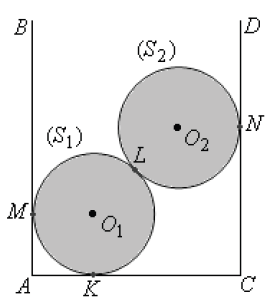
\includegraphics[width=0.9\linewidth]{images/Tc/p2/im1.png}}\\
					\end{center}
					\end{minipage}
					\end{enumerate}}
					\end{exercice}%=== source ===%
  %Exercice 12
\begin{exercice}{}/
					\textbf{نربط كرية حديدية بالطرف السفلي لخيط طرفه العلوي مثبت بحامل (حال 1 ممثلة بالشكل 1).\\
					يوضع مغنطيس بالقرب من الكرية فينحرف الخيط (حالة 2 ممثلة بالشكل 2).
					\begin{center}
					\fbox{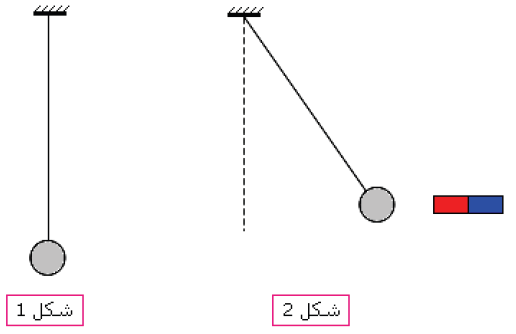
\includegraphics[width=0.5\linewidth]{images/Tc/p2/im2.png}}\\
					\end{center}
					\begin{enumerate}[label=\protect\circled{\color{white}\textbf{\arabic*}}]
					\item أجرد القوى المطبقة على الكرية في الحالة 1 ومثل بدون سلم متجهات القوى في الشكل 1.
					\item أجرد القوى المطبقة على الكرية في الحالة 2 ومثل بدون سلم متجهات القوى في الشكل 2.
					\end{enumerate}}
					\end{exercice}%=== source ===% 
  %Exercice 13
\begin{exercice}{}/
					\textbf{وضع جسم صلب 
					$\bm{(S)}$
					كتلته 
					$\bm{m=1\ kg}$
					على سطح مستوي ومائل بالزاوية 
					$\bm{\alpha=20^o}$
					بالنسبة للمستوى الأفقي.\\
					يلاحظ أن الجسم لا ينزلق على السطح ويبقى في حالة توازن.
					\begin{enumerate}[label=\protect\circled{\color{white}\textbf{\arabic*}}]
					\begin{minipage}[c]{0.59\linewidth}
					\item أجرد القوى المطبقة على 
					$\bm{(S)}$.
					\item بتطبيق شرط توازن جسم صلب خاضع لقوتين بين أن التماس بين 
					$\bm{(S)}$
					والسطح يتم باحتكاك.
					\item حدد شدة 
					$\bm{{\overrightarrow{R}}}$
					المقرونة بتأثير سطح التماس على 
					$\bm{(S)}$
					وقيمة زاوية الإحتكاك 
					 $\bm{\varphi}$.
					 \item استنتج شدة المركبتين المماسية 
					 $\bm{{\overrightarrow{R}_T}}$
					 والمنظمية
					  $\bm{{\overrightarrow{R}_N}}$
					 للقوة
					  $\bm{{\overrightarrow{R}}}$.
					\end{minipage}
					\begin{minipage}[c]{0.39\linewidth}
					\begin{flushleft}
					\fbox{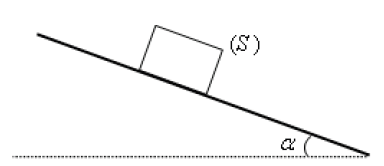
\includegraphics[width=0.9\linewidth]{images/Tc/p2/im3.png}}
					\end{flushleft}
					\end{minipage}
					\end{enumerate}
					نعطي : شدة الثقالة 
					$\bm{g=10\ N.kg^{-1}}$.}
					\end{exercice}%=== source ===%
  %Exercice 14
\begin{exercice}{}/
					\textbf{على سطح مستوي وأفقي، وضع جسم صلب أسطواني الشكل كتلته 
					$\bm{m=10\ kg}$
					وقطر قاعدته 
					$\bm{d=10\ cm}$.\\
					\begin{minipage}[c]{0.69\linewidth}
					\begin{enumerate}[label=\protect\circled{\color{white}\textbf{\arabic*}}]
					\item أحسب شدة القوة الضاغطة التي يطبقها الجسم على سطح التماس.
					\item مثل متجهة القوة الضاغطة باستعمال سلم مناسب.
					\item أحسب قيمة الضعط الذي يطبقه الجسم على سطح التماس.
					\end{enumerate}
					نعطي : شدة الثقالة 
					$\bm{g=10\ N.kg^{-1}}$.
					\end{minipage}
					\begin{minipage}[c]{0.29\linewidth}
					\begin{center}
					\fbox{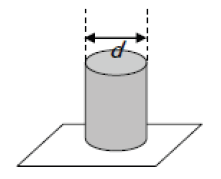
\includegraphics[width=0.9\linewidth]{images/Tc/p2/im4.png}}
					\end{center}
					\end{minipage}}
					\end{exercice}%=== source ===% 
  %Exercice 15
\begin{exercice}{}/
					\textbf{في سائل يتغير الضغط 
					$\bm{p}$
					بدلالة العمق 
					$\bm{h}$
					حسب العلاقة التالية : 
					$\bm{p-p_0=\rho.g.h}$\\
					حيث 
					$\bm{p_0}$
					الضغط الجوي، و
					$\bm{\rho}$
					الكتلة الحجمية للسائل.
					\begin{enumerate}[label=\protect\circled{\color{white}\textbf{\arabic*}}]
					\begin{minipage}[c]{0.59\linewidth}
					\item باستغلال علاقة الضغط بالعمق، فسر لماذا ينبغي أن تكون قاعدة سد أعرض من جزئه العلوي.
					\item أحسب قيمة ضغط الماء عند العمق 
					$\bm{h=60\ m}$.
					\item أحسب شدة القوة الضاغطة المطبقة على غطاء سِكْر له شكل قرص قطره 
					$\bm{d=1,0\ m}$
					عند العمق 
					$\bm{h=60\ m}$.
					\end{minipage}
					\begin{minipage}[c]{0.4\linewidth}
					\begin{flushleft}
					\fbox{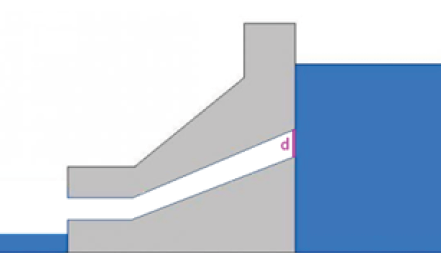
\includegraphics[width=0.8\linewidth]{images/Tc/p2/im5.png}}
					\end{flushleft}
					\end{minipage}
					\end{enumerate}
				نعطي :
					\begin{itemize}
					\item الضغط الجوي :
					$\bm{p_0=1,0.10^5\ Pa}$.
					\item شدة الثقالة : 
					$\bm{g=10\ N.kg^{-1}}$.
					\item الكتلة الحجمية للماء : 
					$\bm{{\rho=1,0.10^3\ kg.m^{-3}}}$.
					\end{itemize}}
					\end{exercice}%=== source ===%  
  %Exercice 16
\begin{exercice}{}/
					\textbf{نقرب عارضة مكهربة من كرية مكهربة فولاذية معلقة بواسطة خيط ثبت طرفه إلى حامل.
					\begin{enumerate}[label=\protect\circled{\color{white}\textbf{\arabic*}}]
					\begin{minipage}[c]{0.64\linewidth}
					\item أجرد القوى المطبقة على الكرية.
					\item صنف هذه القوى إلى قوى تماس و قوى عن بعد وقوى تماس مموضعة و قوى تماس موزعة.
					\item هل هذه القوى داخلية أم خارجية؟
					\item
					 إذا اختيرت المجموعة \{الكرية ، الخيط\} . هل القوة التي يطبقها الخيط على الكرية داخلية أم خارجية؟ علل جوابك.
					\end{minipage}
					\begin{minipage}[c]{0.34\linewidth}
					\begin{flushleft}
					\fbox{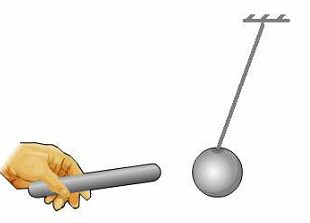
\includegraphics[width=0.9\linewidth]{images/Tc/p2/im6.png}}
					\end{flushleft}
					\end{minipage}
					\end{enumerate}}
					\end{exercice}%=== source ===%
  %Exercice 17
\begin{exercice}{}/
					\textbf{نجر جسما 
					$\bm{(S)}$
					بواسطة خيط غير قابل للتمدد على سطح أفقي ثم على سطح مائل كما يبين الشكل جانبه. \\مثل بدون سلم القوى المطبقة على
					$\bm{(S)}$
					في الحالتين :
					\begin{enumerate}[label=\protect\circled{\color{white}\textbf{\arabic*}}]
					\begin{minipage}[c]{0.34\linewidth}
					\item التماس يتم بدون احتكاك.
					\item التماس يتم باحتكاك.
					\end{minipage}
					\begin{minipage}[c]{0.64\linewidth}
					\begin{flushleft}
					\fbox{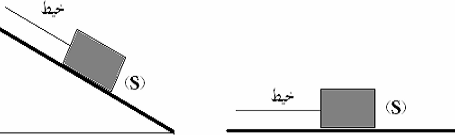
\includegraphics[width=0.9\linewidth]{images/Tc/p2/im7.png}}
					\end{flushleft}
					\end{minipage}
					\end{enumerate}}
					\end{exercice}%=== source ===%
  %Exercice 18
\begin{exercice}{}/
					\textbf{تتكون محقنة أسطوانية الشكل من مكبس شعاعه
					$\bm{R=2\ cm}$
					وتحتوي على غاز محصور بداخلها ضغطه
					$\bm{0,5\ bar}$.
					\begin{enumerate}[label=\protect\circled{\color{white}\textbf{\arabic*}}]
					\item بواسطة تبيانة بسيطة جدا حدد اتجاه القوة الضاغطة المطبقة من طرف الغاز على المكبس.
					\item أحسب شدة هذه القوة.
					\end{enumerate}}
					\end{exercice}%=== source ===%
  %Exercice 19
\begin{exercice}{}/
					\textbf{\textbf{نعتبر عارضة
					$OA$
					  كتلتها
					$M=0,5kg$
						و طولها
					$L=1m$
						قابلة للدوران حول محور
					$\vartriangle$   
					أفقي يمر من طرفها 
					$O$
					ومرتبطة بالطرف الحر
					 $A$ 
					لنابض
					كتلته مهملة و طوله الأصلي 
					$I_0$
					 تكون العارضة زاوية
					 $\alpha$
					  مع الخط المنظمي.
					\begin{center}
					\fbox{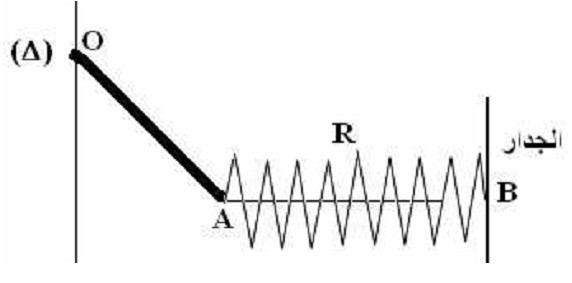
\includegraphics[width=0.5\linewidth]{images/Tc/p2/im8.png}}\\
					\end{center}
					\begin{enumerate}[label=\protect\circled{\color{white}\textbf{\arabic*}}]
					\item 
					نعتبر المجموعة
					 \{نابض ، عارضة OA \} . 
					 أجرد القوى المطبقة على المجموعة، ثم صنفها إلى قوى داخلية و خارجية. ماذا يمكن أن نستنتج
					للقوى الداخلية.
					\item صنف القوى الخارجية إلى قوى التماس و قوى عن بعد ثم إلى قوى التماس
					المموضعة و قوى التماس الموزعة.
					\item مثل على التبيانة متجهة وزن العارضة و متجهة القوة المطبقة من طرف العارضة
					على النابض إذا علمت أن شدتها
					$\bm{6\ N}$.
					السلم
					${4N\longleftrightarrow 1cm}$.
					\item نعتبر المجموعة المدروسة العارضة . أجرد القوى المطبقة على العارضة. مثل على
					تبيانة متجهة القوة المطبقة من طرف النابض على العارضة، غذا علمت أن شدتها
					$6N$.
					استعمل نفس السلم السابق.
					\end{enumerate}}}
					\end{exercice}%=== source ===%
  %Exercice 20
\begin{exercice}{}/
					\textbf{لاحظ الشكل التالي، حيث الكرية
					$\bm{A}$
					مغمورة في الماء. إملأ الجدول التالي بوضع علامة
					$\bm{(\times)}$
					في الخانة المناسبة:
					\begin{minipage}[c]{0.74\linewidth}
					\begin{center}
					 \begin{tabular}{|c|c|c|c|c|c|c|}
					\hline 
					 & نعم & لا & عن بعد & بالتماس & تأثير مموضع & تأثير موزع \\ 
					\hline 
					يؤثر الخيط على $A$ &   &   &   &   &  &  \\ 
					\hline 
					يؤثر الأرض على  $A$ &   &   &   &   &   &   \\ 
					\hline 
					يؤثر الماء على  $A$ &   &   &   &   &   &   \\ 
					\hline 
					يؤثر الحامل على الخيط &   &   &   &   &   &   \\ 
					\hline 
					يؤثر  $A$ على الخيط &   &   &   &   &   &   \\ 
					\hline 
					يؤثر الحامل على  $A$ &   &   &   &   &  &   \\ 
					\hline 
					\end{tabular}
					 \end{center} 
					\end{minipage}
					\begin{minipage}[c]{0.24\linewidth}
					\begin{flushleft}
					\fbox{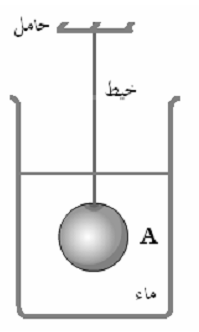
\includegraphics[width=0.6\linewidth]{images/Tc/p2/im9.png}}
					\end{flushleft}
					\end{minipage}}
					\end{exercice}%=== source ===%
  %Exercice 21
\begin{exercice}{}/
					\textbf{يطبق غاز على جزء من إناء مساحته،
					$\bm{S = 25\ cm^{2}}$
					 قوة ضاغطة شدتها 
					 $\bm{F = 375\ N}$. 
					 \begin{enumerate}[label=\protect\circled{\color{white}\textbf{\arabic*}}]
					 \item أحسب قيمة الضغط المطبق من طرف الغاز.
					 \item قارن هذه القيمة بقيمة الضغط الجوي.
					 \item أي تغيير سيطرأ على قيمة لضغط عندما تتضاعف المساحة باعتبار شدة القوة تبقى ثابتة.
					 \end{enumerate}
					\textbf{نعطي :}
					\begin{itemize}
					\item
					الضغط الجوي : 
					{$\bm{P_{atm}=1013\ hPa}$}.
					\end{itemize}}
					\end{exercice}%=== source ===%  
  
\end{document}